%
% teil2.tex -- Beispiel-File für teil2 
%
% (c) 2020 Prof Dr Andreas Müller, Hochschule Rapperswil
%
% !TEX root = ../../buch.tex
% !TEX encoding = UTF-8
%
\section{Riemannsche Zeta-Funktion}\label{Riemannsche Zeta-Funktion}
\kopfrechts{Riemannsche Zeta-Funktion}

Die riemannsche Zeta-Funktion wurde 1859 von Bernhard Riemann untersucht und ist eine zentrale Funktion der
\index{Bernhard Riemann}%
\index{Riemann, Bernhard}%
analytischen Zahlentheorie. Sie wird üblicherweise als unendliche Reihe
\index{analytische Zahlentheorie}%
definiert. Für alle komplexen Variablen $s$ mit Realteil grösser als 1 ergibt sich ihre Darstellung als
\[
\zeta(s) = \sum_{n = 1}^{\infty}\frac{1}{n^{s}}.
\]
Diese Definition beschreibt eine Dirichlet-Reihe, deren Konvergenz für $\operatorname{Re}(s) > 1$ gewährleistet ist. 
Bereits in diesem Definitionsbereich zeigt die Funktion bemerkenswerte Eigenschaften. 
So nimmt sie für bestimmte Argumente konkrete Werte an, wie in Tabelle \ref{tab:zeta} dargestellt ist.

%
% table.tex -- Tabelle der Zeta-Werte
%
% (c) 2026 Prof Dr Andreas Müller
%
\begin{table}
\centering
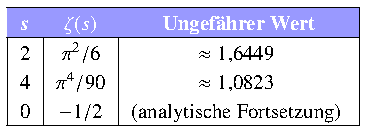
\includegraphics{papers/zeta/images/tabular.pdf}
\caption{Ausgewählte Werte der Zeta-Funktion}
\label{tab:zeta}
\end{table}


Besonders bemerkenswert ist hier der Wert $\zeta$(2) = $\frac{\pi^2}{6}$, den Euler bereits 1735 nachwies, bekannt als das Basler Problem (siehe Kapitel \ref{chapter:basel}).
\index{Euler, Leonhard}%
\index{Basel-Problem}%
Die letze Zeile der Tabelle gehört jedoch nicht zum ursprünglichen Definitionsbereich (s > 1), sondern ist nur durch analytische Fortsetzung erreichbar. 

Bereits der Fall $s = 0$ zeigt, dass es sich bei solchen divergenten Werten nicht um Einzelfälle handelt.
Setzt man $s = 0$ formal in die Reihendefinition ein, so erhält man
\[
\zeta(0) \overset{?}{=} \sum_{n=1}^{\infty} 1 = 1 + 1 + 1 + \ldots,
\]
also genau die in Abschnitt~\ref{konvergente-und-divergente-reihen} als bestimmt divergent identifizierte Reihe.
Dennoch liefert die analytische Fortsetzung dafür den wohldefinierten Wert $\zeta(0) = -1/2$ (vgl. Tabelle~\ref{tab:zeta}).
Das deutet darauf hin, dass hinter solchen Werten eine globale, einheitliche Methode steht und nicht eine Sammlung von Einzelfällen, die man je einzeln erklären müsste.

Ein besonders interessanter Fall ist $s = -1$, mit dem wir uns im weiteren Verlauf dieses Papers eingehender beschäftigen.
Setzt man diesen Wert formal in die Reihendefinition ein, so erhält man
\[
\zeta(-1) \overset{?}{=} \sum_{n=1}^{\infty} \frac{1}{n^{-1}} = \sum_{n=1}^{\infty} n = 1 + 2 + 3 + \ldots,
\]
also genau die Summe aller natürlichen Zahlen.
Dieses Einsetzen ist jedoch nicht zulässig: Die Reihe $\sum_{n=1}^{\infty} n^{-s}$ konvergiert nur für $\operatorname{Re}(s) > 1$, für $s = -1$ ist sie schlicht divergent und die Reihendefinition liefert keinen Wert.
Der Wert von $\zeta(-1)$ kann also nicht direkt aus der Reihe berechnet werden, sondern muss auf anderem Weg gewonnen werden.
Wie dies mit Hilfe der analytischen Fortsetzung gelingt, wird in Abschnitt~\ref{Analytische Fortsetzung} gezeigt.

\begin{figure}
	\centering
	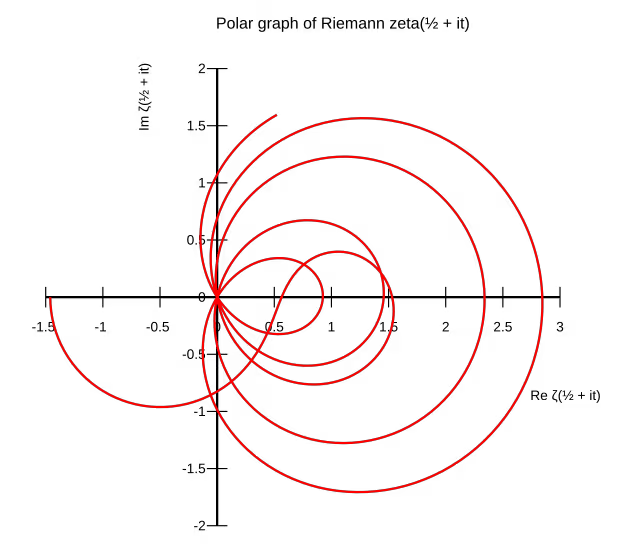
\includegraphics[width=1.0\linewidth]{papers/zeta/Abbildung_Zeta.png}
	\caption{Werte der riemannschen Zeta-Funktion auf der kritischen Geraden $\operatorname{Re}(s) = \frac{1}{2}$, dargestellt als Polarkurve $\zeta\bigl(\frac12 + it\bigr)$ für variierendes $t$.}
	\label{fig:abbildungzeta}
\end{figure}

Die spiralförmige Darstellung in Abbildung \ref{fig:abbildungzeta} zeigt die Werte der Zeta-Funktion $\zeta(s)$ auf der kritischen Geraden $\operatorname{Re}(s) = \frac{1}{2}$, das heisst für $s = \frac12 + it$ mit variierendem reellen Parameter $t$. Die Schnittpunkte der Kurve mit dem Ursprung (sichtbar als die Stellen, an denen die Spirale durch den Mittelpunkt verläuft) entsprechen den sogenannten nicht-trivialen Nullstellen der Zeta-Funktion, die auf dieser Geraden liegen. Dass tatsächlich alle nicht-trivialen Nullstellen auf der Linie $\operatorname{Re}(s) = \frac{1}{2}$ liegen, ist Gegenstand der berühmten, bis heute unbewiesenen riemannschen Vermutung, einem der bedeutendsten offenen Probleme der Mathematik.
\index{kritische Gerade}%

Nützlich ist die riemannsche Zeta-Funktion ebenfalls, um eine Annäherung der Primzahlfunktion zu schaffen. 
Das Euler-Produkt
\[
\zeta(s) = \prod_{p \ \text{prim}} \frac{1}{1 - p^{-s}}
\]
beschreibt eine geometrische Reihe, welche den Zusammenhang aller Primzahlen aufzeigt. 

\begin{figure}
	\centering
	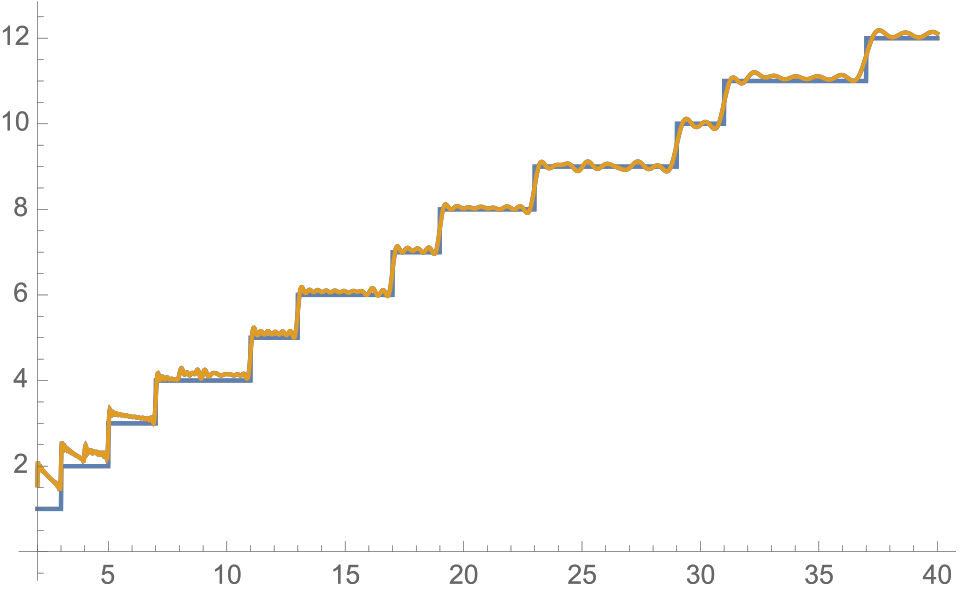
\includegraphics[width=0.7\linewidth]{papers/zeta/Primzahlen.png}
	\caption{Primzahlzählfunktion}
	\label{fig:primzahlen}
\end{figure}

Die blaue Treppenkurve in Abbildung~\ref{fig:primzahlen} zeigt die Primzahlzählfunktion $\pi(x)$, welche für jede reelle Zahl $x$ angibt, wie viele Primzahlen kleiner oder gleich $x$ existieren.
\index{Primzahlzählfunktion}%
Die orangefarbene Kurve stellt den logarithmischen Integralausdruck $\operatorname{Li}(x)$ dar, eine glatte, sprungfreie Funktion. Er wird in Definition \ref{buch:intalg:risch:def:integrallogarithmus} eingeführt.
Das ist eine von Riemann entwickelte Näherungsformel für $\pi(x)$, die direkt aus der Zeta-Funktion abgeleitet wird. Eine ausführliche, gut nachvollziehbare Herleitung deses Zusammenhangs findet sich bei \cite{edwards1974riemann}.
Man erkennt, wie eng beide Kurven beieinander liegen: $\operatorname{Li}(x)$ approximiert die Verteilung der Primzahlen, wobei die relative Genauigkeit dieser Näherung mit wachsendem $x$ zunimmt.

